\documentclass{a4beamer}
%% Lectures - common definitions

\usextensions{tikz}
\usetikzlibrary{shapes.multipart,shapes.callouts,shapes.geometric}
\input{fix-callouts.inc} % Fixes absolute positioning of rectangle callouts

\newif\ifbigpages \bigpagesfalse
\ifdim\paperwidth >20cm
	\bigpagestrue
\fi

\tikzset{%
	note/.style={rectangle callout,draw=none,callout pointer width=1em,%
		align=flush left,font=\footnotesize,inner sep=0.5em,%
		fill=blue!15,fill opacity=0.95,text opacity=1.0,callout absolute pointer=#1},
	node distance=2em and 2.75em
}
\ifbigpages
	% Scale all arrow tips by the factor of 2.5
	\let\old@pgf@arrow@call=\pgf@arrow@call
	\def\pgf@arrow@call#1{%
		\@tempdima=\pgflinewidth%
		\pgfsetlinewidth{2.5\pgflinewidth}%
		\old@pgf@arrow@call{#1}%
		\pgfsetlinewidth{\@tempdima}%
	}
	\def\pgfarrowsleftextend#1{\pgfmathsetlength{\pgf@xa}{1.5*#1}}
	\def\pgfarrowsrightextend#1{\pgfmathsetlength{\pgf@xb}{1.5*#1}}
\fi

%% Load listings package
\usepackage{listings}

%% Are we inside a comment?
\newif\iflstcomment \lstcommentfalse

\lstset{%
	tabsize=4,
	showstringspaces=false,
	basicstyle=\linespread{1.25}\ttfamily\small,
	keywordstyle=\bfseries,
	commentstyle=\lstcommentstyle,
	numbers=left,
	numberstyle=\footnotesize\color{gray},
	xleftmargin=2.5em,
	extendedchars=true,
	escapechar=\$,
	escapebegin=\iflstcomment\begingroup\lstcommentstyle\fi,
	escapeend=\iflstcomment\endgroup\fi
}

\def\lstcommentstyle{\color{gray}}

\lst@AddToHook{AfterBeginComment}{\global\lstcommenttrue}
\let\orig@lst@EndComment=\lst@EndComment
\def\lst@EndComment{\global\lstcommentfalse\orig@lst@EndComment}
\lst@AddToHookAtTop{EOL}{%
	\lst@ifLmode\global\lstcommentfalse\fi% XXX Sloppy way to determine comment end
}

%% Python with docstrings treated as comments
\lstdefinelanguage[doc]{python}[]{python}{%
	deletestring=[s]{"""}{"""},%
	morecomment=[s]{"""}{"""}%
}%

%% JavaScript language
\lstdefinelanguage{javascript}%
	{morekeywords={break,case,catch,%
		const,constructor,continue,default,do,else,false,%
		finally,for,function,if,in,instanceof,%
		new,null,prototype,%
		return,switch,this,throw,%
		true,try,typeof,var,while},%
	sensitive,%
	morecomment=[l]//,%
	morecomment=[s]{/*}{*/},%
	morestring=[b]",%
	morestring=[b]',%
}[keywords,comments,strings]%

%% C# language (4.0?)
\lstdefinelanguage{csharp}%
	{morekeywords={abstract,as,%
		base,bool,byte,case,catch,char,%
		checked,class,const,continue,%
		decimal,default,delegate,do,double,%
		else,enum,event,explicit,extern,%
		false,finally,fixed,float,for,foreach,%
		goto,if,implicit,in,int,interface,%
		internal,is,lock,long,%
		namespace,new,null,object,operator,out,%
		override,params,private,protected,public,%
		readonly,ref,return,sbyte,sealed,%
		short,sizeof,stackalloc,static,string,%
		struct,switch,this,throw,true,try,%
		typeof,uint,ulong,unchecked,unsafe,ushort,%
		using,virtual,void,volatile,while%
	},%
	sensitive,%
	morecomment=[l]//,%
	morecomment=[s]{/*}{*/},%
	morestring=[b]",%
	morestring=[b]',%
}[keywords,comments,strings]%

%% Translation for fact environment
\deftranslation[to=russian]{Fact}{Наблюдение}

%% Inline code snippets
\def\code#1{\texttt{#1}}
\def\codekw#1{\code{\textbf{#1}}}

\def\quoteauthor#1{\par\footnotesize\upshape\hfill—~#1}

%% English term
\def\engterm#1{(англ. \textit{#1})}
%% Term with explanation below (to be used in diagrams)
\def\termwithexpl#1#2{#1\strut{}\\\small\color{gray}(\textit{#2})\strut{}}
%% External link
\def\extlink#1#2{\href{#1}{\color[rgb]{0.7,0.7,1.0}\dashbar{#2}}}
%% Internal link
\def\inlink#1#2{\hyperlink{#1}{\color[rgb]{0.7,0.7,1.0}\dashbar{#2}}}
%% Explanation for a list item
\def\itemexpl#1{\begingroup\small\vspace{0.75ex}#1\par\endgroup}



\usetikzlibrary{decorations.pathreplacing}


\lecturetitle{Программная инженерия. Лекция №16 — Документирование ПО}
\title[Документирование]{Документирование ПО}
\author{Алексей Островский}
\institute{\small{Физико-технический учебно-научный центр НАН Украины}\vspace{2ex}}
\date{26 марта 2015 г.}

\begin{document}
	\frame{\titlepage}

	\section{Общие понятия}

	\frame{
		\frametitle{Документация на ПО}

		\begin{Definition}
		\textbf{Документация} — печатный текст, сопровождающий программное обеспечение для~объяснения 
		принципов его функционирования или использования.
		\end{Definition}

		\vspace{1ex}
		\textbf{Цели документирования:}
		\begin{itemize}
			\item посредничество между разработчиками ПО;
			\item упрощение сопровождения и эволюции;
			\item информация для планирования и оценки затрат в процессе разработки;
			\item инструкции по использованию и управлению программной системой;
			\item основание для сертификации системы.	
		\end{itemize}
	}

	\frame{
		\frametitle{Документация на ПО}

		\begin{center}
			\begin{tikz*}[%
	every node/.style={rectangle,align=center,minimum height=3.25em,minimum width=8.5em}
]
	\node(req) [draw] {Инженерия \\ требований};
	\node(req-doc) [right=5em of req] {Спецификация \\ требований};
	\node(design) [below=of req,draw] {Проектирование};
	\node(des-doc) at (req-doc.south |- design.east) {архитектурная / проектная \\ документация};
	\node(impl) [below=of design,draw] {Имплементация};
	\node(impl-doc) at (req-doc.south |- impl.east) {Техническая \\ документация};
	\node(test) [below=of impl,draw] {Тестирование};
	\node(maint) [below=of test,draw] {Сопровождение};
	
	\draw[->] (req) to (design);
	\draw[->,dashed] (req) to (req-doc);
	\draw[->] (design) to (impl);
	\draw[->,dashed] (design) to (des-doc);
	\draw[->] (impl) to (test);
	\draw[->,dashed] (impl) to (impl-doc);
	\draw[->] (test) to (maint);

	\draw[decorate,decoration={brace,amplitude=0.4em,raise=5pt}] (req.west |- test.west) 
		-- node[left,minimum width=12em] {Пользовательская \\ документация; \\ маркетинговая \\ документация} (req.west);
\end{tikz*}


			\figureexpl{Документирование в процессе разработки ПО}
		\end{center}
	}

	\subsection{Типы документации}

	\frame{
		\frametitle{Типы документации}

		Документация \textbf{на процесс разработки} \engterm{process documentation}:
		\begin{itemize}
			\item планы разработки;
			\item расписания;
			\item документы оценки качества процессов разработки;
			\item организационные и проектные стандарты.
		\end{itemize}

		\vspace{1ex}
		Документация \textbf{на продукты разработки} \engterm{product documentation}:
		\begin{itemize}
			\item
			системная (техническая) документация — описание программной системы с~точки~зрения разработчика;
			\item
			пользовательская документация — описание~ПО с~точки~зрения конечного пользователя.
		\end{itemize}
	}

	\subsection{Документация в гибкой методологии}

	\frame{
		\frametitle{Документация в гибкой методологии}

		\begin{quote}
			\begin{center}Работающее ПО \quad $>$ \quad Исчерпывающая документация\end{center}

			\figureexpl{\hfill— Agile Manifesto}
		\end{quote}

		\vspace{1ex}
		\textbf{Недостатки традиционного подхода} к документированию:
		\begin{itemize}
			\item
			Производство документации и поддержка документов в актуальном состоянии 
			занимает много времени и средств и приводит к замедлению процесса разработки.
			\item
			Требования к ПО меняются настолько быстро, что документация устаревает практически сразу после написания.
		\end{itemize}

		\vspace{1ex}
		\textbf{Необходимые виды документации:}
		\begin{itemize}
			\item пользовательская документация;
			\item обоснование архитектурных решений;
			\item документация критических систем.
		\end{itemize}
	}

	\subsection{Структура документации}

	\frame{
		\frametitle{Структура документации}

		\textbf{Основной стандарт:} IEEE 1063 — Standard for Software User Documentation [2001].

		\vspace{1ex}
		\textbf{Структура документации на ПО:}
		\begin{enumerate}
			\item
			данные, позволяющие идентифицировать документ (заголовок, дата составления и~т.\,п.);
			\item
			содержание;
			\item
			список иллюстраций и таблиц (опционально);
			\item
			введение — назначение документа и краткое описание содержимого;
			\item
			информация по использованию — советы по эффективному использованию 
			различными группами пользователей (новичками, опытными пользователями, администраторами, …);
		\end{enumerate}
	}

	\frame{
		\frametitle{Структура документации}

		\textbf{Структура документации на ПО} (продолжение):
		\begin{enumerate}
			\setcounter{enumi}{5}
			\item
			концепция ПО — описание вариантов использования программной системы;
			\item
			команды — описание команд, поддерживаемых системой;
			\item
			выдаваемые программой сообщения об ошибках и способы их устранения;
			\item
			словарь используемых в документе специфичных терминов;
			\item
			связанные документы и информационные ресурсы;
			\item
			навигация (особенно для электронных документов);
			\item
			алфавитный указатель по командам;
			\item
			поиск по содержанию (для электронных документов).
		\end{enumerate}
	}

	\subsection{Стиль документации}

	\frame{
		\frametitle{Стиль документации}

		\begin{itemize}
			\item
			Предпочтительно использование английского языка, в т.\,ч. из-за проблем перевода терминов;
			\item
			проверка грамматики (присутствует в современных средах разработки);
			\item
			короткие и ясные предложения; короткие абзацы (не более 7 предложений).
			\item
			четкие определения для используемых терминов;
			\item
			нумерованные и ненумерованные списки для перечислений, выделение текста (курсив или~полужирное начертание);
			\item
			заголовки и подзаголовки для фрагментации информации;
			\item
			иллюстрации и таблицы для наглядности.
		\end{itemize}
	}

	\subsection{Форматы документации}

	\frame{
		\frametitle{Форматы документации}

		\begin{itemize}
			\item
			\textbf{Печатная документация};

			\vspace{1ex}
			\item
			\textbf{Электронная документация:}
			\begin{itemize}
				\item
				локальные файлы (plain text, Markdown, HTML, PDF, …);
				\item
				интегрируемая в общесистемную справочную систему (man, info, …);
				\item
				интегрируемая в среду разработки (напр., исходные Java-файлы или~javadoc-архивы 
				при~разработке на~Java в~Eclipse).
			\end{itemize}

			\vspace{1ex}
			\item
			\textbf{Онлайн-документация:}
			\begin{itemize}
				\item
				поддерживаемая разработчиком (руководство по установке / Getting started / справочные руководства, …);
				\item
				Web 2.0-документация, поддерживаемая пользователями (wiki, блоги, вопросы на~\extlink{http://stackoverflow.com/}{stackoverflow}, …)
			\end{itemize}
		\end{itemize}
	}

	\frame{
		\frametitle{Онлайн-документация}

		\textbf{Преимущества:}
		\begin{itemize}
			\item
			доступность для потребителей, актуальность документации;
			\item
			гипертекстовая связанность в пределах документации и с другими источниками информации;
			\item
			больший объем документов;
			\item
			веб 2.0 — возможность комментирования документации, обмена опытом с~другими пользователями ПО.
		\end{itemize}

		\vspace{1ex}
		\textbf{Недостатки:}
		\begin{itemize}
			\item
			усложнение поиска по нечетким запросам;
			\item
			ухудшение воспринимаемости текста;
			\item
			большой объем малополезной информации.
		\end{itemize}
	}

	\section{Виды документации}

	\subsection{Документирование процессов разработки}

	\frame{
		\frametitle{Документирование процессов разработки}

		\textbf{Виды документации:}
		\begin{itemize}
			\item
			планы, оценки затрат и расписания: составляются менеджерами для управления процессом разработки;

			\vspace{1ex}
			\item
			отчеты: использование ресурсов на различных этапах;

			\vspace{1ex}
			\item
			стандарты: ограничения на процесс разработки (специфичные для организации или национальные / международные);

			\vspace{1ex}
			\item
			рабочие документы (working paper): особенности архитектуры системы, стратегии имплементации;

			\vspace{1ex}
			\item
			общение между разработчиками и менеджерами.
		\end{itemize}
	}

	\frame{
		\frametitle{Объем документации на процесс разработки}

		\begin{fact}
			Большая часть документации на процесс разработки может быть заменена 
			неформальными дискуссиями между разработчиками, менеджерами и заказчиком.
		\end{fact}

		\vspace{1ex}
		\textbf{Необходимая документация на процесс разработки:}
		\begin{itemize}
			\item явно определенная договором с заказчиком;
			\item необходимая для сертификации системы;
			\item расписание тестирования (заменяется автоматическими тестами);
			\item рабочие документы (могут быть выделены в отдельные статьи).
		\end{itemize}
	}

	\subsection{Пользовательская документация}

	\frame{
		\frametitle{Пользовательская документация}

		\begin{Definition}
		\textbf{Пользовательская документация} \engterm{user documentation} — документы, 
		описывающие использование программной системы конечными пользователями.
		\end{Definition}

		\vspace{1ex}
		\textbf{Организация пользовательской документации:}
		\begin{itemize}
			\item
			учебные пособия — описание шагов для решения определенных задач с помощью программной системы;
			\item
			темы — объединение логически связанных документов в главы / разделы, описывающие определенный аспект ПО;
			\item
			справочники — перечень выполняемых системой функций.
		\end{itemize}
	}

	\frame{
		\frametitle{Виды пользовательской документации}

		\begin{center}\small
			\begin{tabular}{|p{0.22\textwidth}|p{0.3\textwidth}|p{0.3\textwidth}|}
				\hline
				\centering Вид & \centering Потребители & \centering Содержание \cr
				\hline
				\raggedright Функциональное описание системы & \raggedright менеджеры, заказчик 
					& \raggedright обзор системы, описание отличительных особенностей \cr
				\hline
				\raggedright Руководство по~установке & \raggedright системные администраторы 
					& \raggedright описание этапов установки системы \cr
				\hline
				\raggedright Введение \engterm{getting started} & пользователи 
					& \raggedright краткое руководство для~начального знакомства с~системой \cr
				\hline
				\raggedright Справочное руководство \engterm{reference manual} & \raggedright опытные пользователи 
					& \raggedright детальное описание функционала~ПО \cr
				\hline
			\end{tabular}
		\end{center}
	}

	\subsection{Системная документация}

	\frame{
		\frametitle{Системная документация}

		\begin{Definition}
			\textbf{Системная документация} \engterm{system documentation} — документы, 
			описывающие структуру программной системы.
		\end{Definition}

		\vspace{1ex}
		\textbf{Виды системной документации:}
		\begin{itemize}
			\item документ спецификации требований;
			\item описание общей архитектуры системы;
			\item описание отельных компонентов (архитектура, предоставляемая функциональность и~интерфейсы);
			\item исходный код и комментарии в нем;
			\item документы, касающиеся валидации системы;
			\item руководство по сопровождению системы (известные проблемы, направления эволюции, внешние зависимости, …).
		\end{itemize}
	}

	\subsection{Генерация документации}

	\frame{
		\frametitle{Генерация документации}

		\begin{center}
			\begin{tikz*}[%
	every node/.style={rectangle,draw,align=center,minimum height=3.25em,minimum width=8.5em}
]
	\node(src) {Исходный код};
	\node(comments) [below left=2em and 0em of src] {Комментарии};
	\node(struct) [below right=2em and 0em of src] {Структура};
	\node(gen) [below=of comments] {Генератор \\ документации};
	\node(output) [below=3em of gen,anchor=north] {HTML-страницы, PDF, \\ UML-схемы, …};
	\node(parser) [below=of struct] {Синтаксический \\ анализатор IDE};
	\node(help) [below=3em of parser,anchor=north] {Контекстная \\ помощь};

	\draw[->] (src) -- (comments);
	\draw[->] (src) -- (struct);
	\draw[->] (comments) -- (gen);
	\draw[->] (struct) -- (gen);
	\draw[->] (comments) -- (parser);
	\draw[->] (struct) -- (parser);
	\draw[->] (gen) -- (output);
	\draw[->] (parser) -- (help);
\end{tikz*}


			\vspace{1ex}
			\figureexpl{Генерация документации на основе исходного кода}
		\end{center}
	}

	\frame{
		\frametitle{Генерация документации}

		\textbf{Этапы генерации документации ($\sim$ MVC):}
		\begin{enumerate}
			\item
			определение используемых представлений для исходных файлов;
			\item
			создание синтаксического дерева для исходных файлов;
			\item
			создание моделей для элементов программы (классов, методов, ...);
			\item
			генерация представления на основе моделей (напр., HTML-страниц).
		\end{enumerate}

		\vspace{1ex}
		\textbf{Примеры генераторов документации:}
		\begin{itemize}
			\item Javadoc (основной для Java);
			\item Sphinx (основной для Python);
			\item Doxygen (основной для С / С++).
		\end{itemize}
	}

	\frame{
		\frametitle{Пример документации: Javadoc}

		\begin{itemize}
			\item
			Для составления документации используются комментарии к классам, полям, методам вида \code{/** … */}.

			\vspace{1ex}
			\item
			Для секционирования комментариев применяются теги:
			\begin{itemize}
				\item\code{@param} — для описания параметров методов;
				\item\code{@return} — для описания возвращаемого значения метода;
				\item\code{@throws} — для условий порождения исключений;
				\item\code{@since} — для установления версии ПО, в которой появился класс / метод.
			\end{itemize}

			\vspace{1ex}
			\item
			Для маркировки применяются HTML-теги.

			\vspace{1ex}
			\item
			Теги \code{@link}, \code{@see} позволяют ссылаться на другие элементы документации.
		\end{itemize}
	}

	\frame{
		\frametitle{Пример документации: Javadoc}

		\lstinputlisting[language=java]{code-doc.java}
	}

	\frame{
		\frametitle{Пример документации: Javadoc}

		\begin{center}
			\ifbigpages
				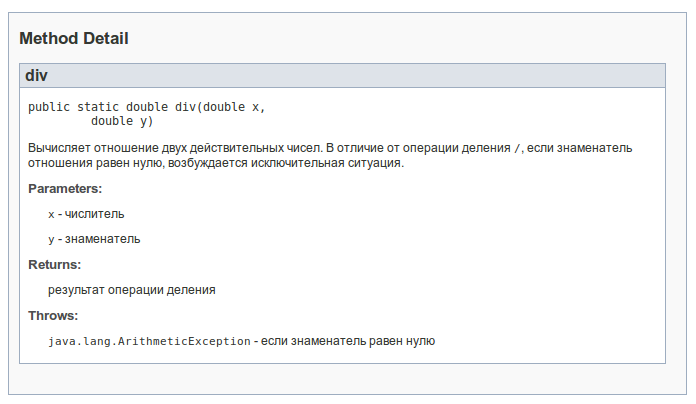
\includegraphics[scale=1]{fig-doc-html.png}
			\else
				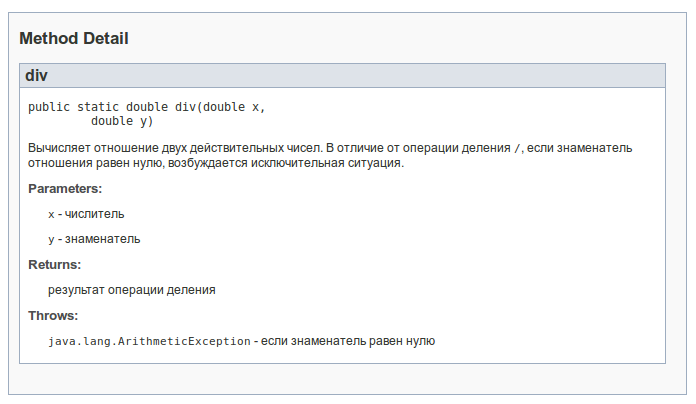
\includegraphics[scale=0.5]{fig-doc-html.png}
			\fi

			\figureexpl{Фрагмент сгенерированной утилитой Javadoc HTML-страницы документации, 
				соответствующей приведенному методу.}
		\end{center}
	}

	\frame{
		\frametitle{Пример документации: Javadoc}

		\begin{center}
			\ifbigpages
				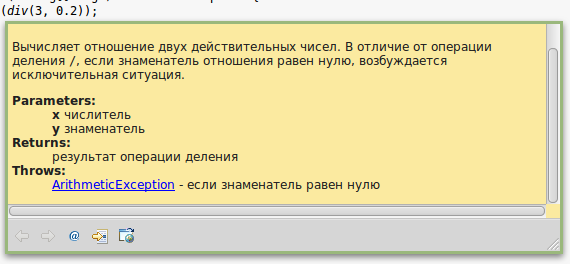
\includegraphics[scale=1]{fig-doc-eclipse.png}
			\else
				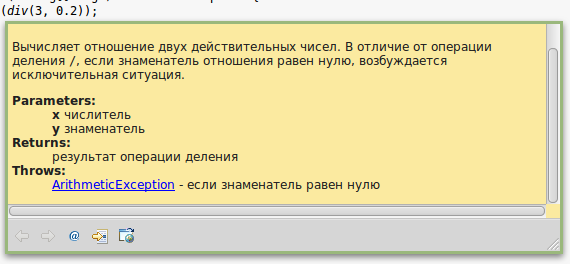
\includegraphics[scale=0.75]{fig-doc-eclipse.png}
			\fi

			\figureexpl{Контекстная помощь для приведенного метода в среде разработки Eclipse.}
		\end{center}
	}

	\subsection{Грамотное программирование}

	\frame{
		\frametitle{Грамотное программирование}

		\begin{Definition}
			\textbf{Грамотное программирование} \engterm{literate programming} — методология программирования и~документирования кода, 
			согласно которой программа (\emph{эссе}) состоит из~текста на~естественном языке с~вкраплениями кода на~языках программирования, 
			возможно с~макроподстановками.
		\end{Definition}

		\vspace{1ex}
		\textbf{Автор:} Дональд Кнут [1981, для системы компьютерной верстки \TeX].

		\vspace{1ex}
		\textbf{Принципы:}
		\begin{itemize}
			\item
			конструирование эссе происходит в порядке разработки программы программистом и~следует его~мысли;

			\item
			роль абстракций выполняют макросы (логически связанные фрагменты кода);

			\item
			«чистый» код программы генерируется препроцессором, обрабатывающим макросы; 
			одному эссе может соответствовать несколько программ, в~т.\,ч. на~разных~ЯП.
		\end{itemize}
	}

	\frame{
		\frametitle{Пример грамотного программирования}

		\textbf{Пример в системе \extlink{https://en.wikipedia.org/wiki/Noweb}{noweb}:}
		\lstinputlisting[language=c,escapechar=\`]{code-noweb.nw}
	}

	\section{Заключение}

	\subsection{Выводы}
	
	\frame{
		\frametitle{Выводы}

		\begin{enumerate}
			\item
			Документация на ПО нужна, чтобы описать его~функционал для~пользователей (пользовательская документация) 
			и~упростить сопровождение и~эволюцию (системная документация).

			\vspace{0.5ex}
			\item
			Согласно гибкой методологии разработки, объем документации (в~особенности документов, описывающих процесс разработки) 
			должен быть сведен к минимуму.

			\vspace{0.5ex}
			\item
			Стандарт IEEE 1063 содержит рекомендации по составлению документации к~ПО, 
			в~частности, приблизительную структуру документов.

			\vspace{0.5ex}
			\item
			Создание документации можно автоматизировать за счет использования генераторов документации наподобие javadoc.
		\end{enumerate}
	}
	
	\subsection{Материалы}
	
	\frame{
		\frametitle{Материалы}
		
		\begin{thebibliography}{9}
			\bibitem[1]{1}
			Sommerville, Ian
			\newblock Software Engineering. Documentation
			\newblock {\footnotesize \extlink{http://ifs.host.cs.st-andrews.ac.uk/Books/SE9/WebChapters/PDF/Ch_30\%20Documentation.pdf}{Доступна по Интернету}.}

			\bibitem[2]{2}
			IEEE Society
			\newblock IEEE 1063 Standard for Software User Documentation
		\end{thebibliography}
	}
	
	\frame{
		\frametitle{}
		
		\begin{center}
			\Huge Спасибо за внимание!
		\end{center}
	}
\end{document}
